\section[UI]{User Interface}
% Første parameter i [] er tekst i header. {} er i indholdsfortegnelsen.

% Slide med emneoverskrift.
\begin{frame}
  \frametitle{}
  \begin{center}
    {\Huge User Interface}
  \end{center}
\end{frame}
\note{
  \begin{itemize}
		\item Introduce
    \item Design choices
    \item Testing
    \item Demo
  \end{itemize}
}

\begin{frame}
    \frametitle{The Design Process}
    \framesubtitle{Starting the process}
    \begin{itemize}
    	\item Design from requirements
    	\item Incremental development
    \end{itemize}
\end{frame}
\note{
	\begin{itemize}
    \item Use Web Engneering Techniques.
    \item built on requirement engineering.
    \item Little by Little.
    \item Fit well with project.
	\end{itemize}
}

\begin{frame}
    \frametitle{The Design Process}
    \framesubtitle{Gathering requirements}
    \begin{itemize}
    	\item Information Flow Diagram
    \end{itemize}
    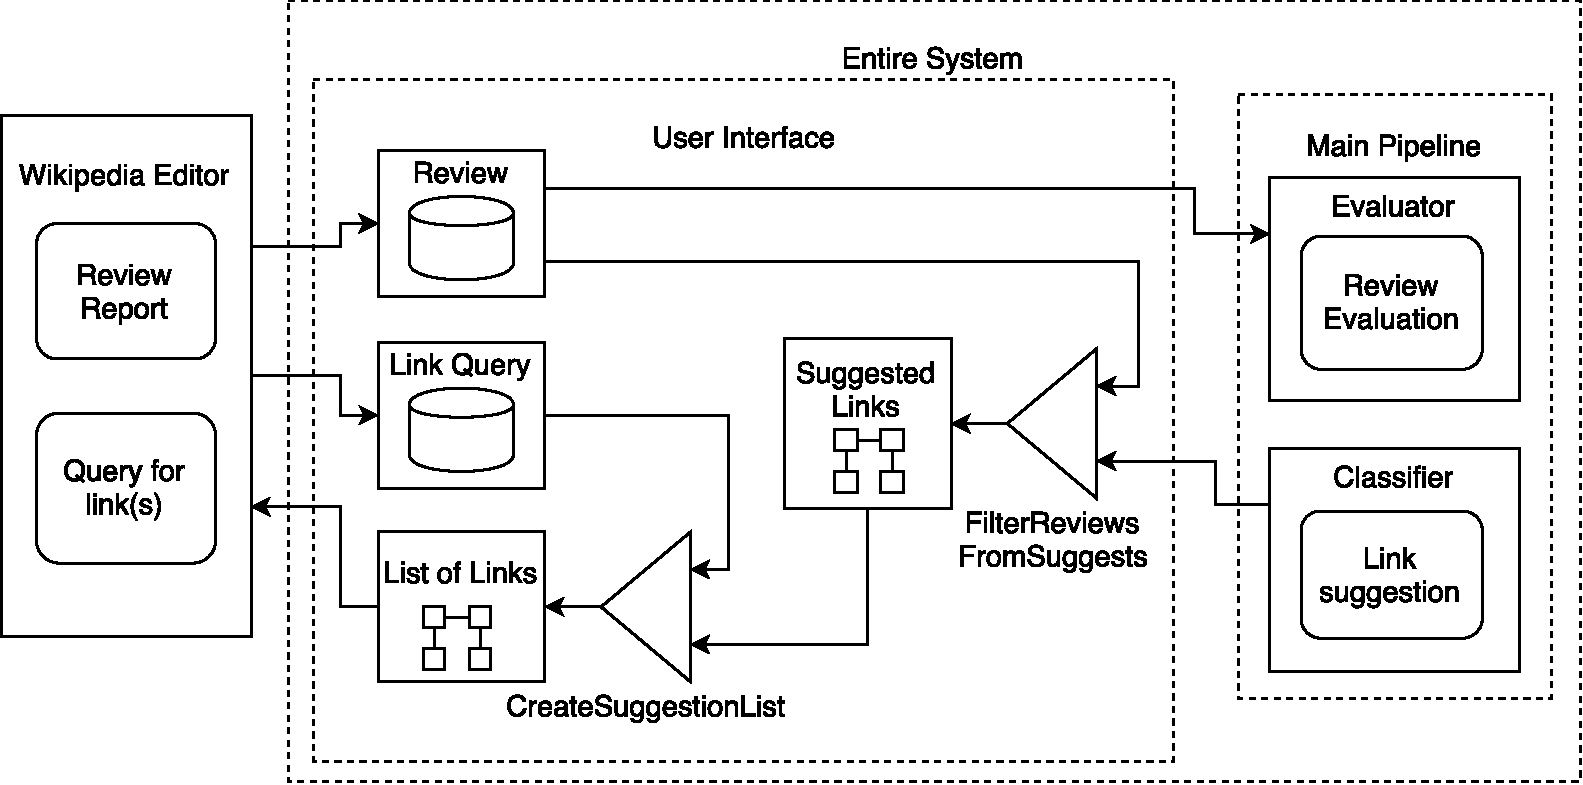
\includegraphics[width=\textwidth]{wikiAPI.pdf}
\end{frame}
\note{
	\begin{itemize}
    \item Organizational Concerns.
    \item Information Delivery.
    \item Understanding our model wishes.
    \item Diagram
    \item Incremental -> simple editors
    \item Created two requirements
	\end{itemize}
}

\begin{frame}
    \frametitle{The Design Process}
    \framesubtitle{Gathering Requirements}
    \begin{itemize}
    	\item A user must be able to query the UI for link suggestions.
    	\item A user should be able to submit reviews of link suggestions.
    \end{itemize}
\end{frame}
\note{
	\begin{itemize}
    \item First and foremost
    \item Secondly -> reaction
    \item learn from it.
	\end{itemize}
}

\begin{frame}
    \frametitle{The Design Process}
    \framesubtitle{Creating a Solution}
    \begin{itemize}
    	\item User Demographic    
    	\item API > GUI
    \end{itemize}
\end{frame}
\note{
	\begin{itemize}
    \item Create Solution Idea
    \item STEP1: Analyze TARGET
    \item Speculation NO CONTACT
    \item Bacbone -> influence
    \item ----------
    \item Reasearch -> API
    \item access as possible
    \item direct GUI
    \item API = Broad dev
    \item realistic
    \item no initiation?
	\end{itemize}
}

\begin{frame}
    \frametitle{Testing the API}
    \framesubtitle{}
    \begin{itemize}
    	\item Unit testing
    	\item Acceptance test
    \end{itemize}
\end{frame}
\note{
	\begin{itemize}
    \item integrity
    \item Django helps
    \item Presedence
	\end{itemize}
}

\begin{frame}
  \frametitle{}
  \begin{center}
    {\Huge DEMO}
  \end{center}
\end{frame}
\note{
  \begin{itemize}
		\item Notes...
  \end{itemize}
}

% \begin{frame}
%     \frametitle{Some Example Title}
%     \framesubtitle{Some example subtitle}
%     \centering
%     Some text, content, etc.
% \end{frame}
% \note{
% 	\begin{itemize}
%     \item Notes here...
% 	\end{itemize}
% }